\section{Evaluation}
\label{res_overview}
 
\begin{table*}
\centering
\caption{Evaluation results overview. We evaluate two versions of mbedTLS and five
versions of OpenSSL\@. CF represents secret-dependent control-flow transfers and
DF represents secret-dependent data-flow transfers. Side-channel leakagas can
be found by symbolic execution and we run Monte Carlo to estimate the amount 
of leakage information. A summary of all vulnerabilities with the amount of
leak information can be found in the appendix.
}\label{fig:Testtt}
\begin{tabular}{clrrrrrrr}
\hline
\textbf{Algorithm} & \textbf{Implementation} & \textbf{Lekage Sites} & \textbf{CF} & \textbf{DF}
& \textbf{\# Instructions} & \textbf{Max Leakeage} & \textbf{Sym.\ Exe.} & \textbf{Monte Carlo}\\\hline
&&&&&& bits & ms & ms\\\cline{7-9}
AES & mbed TLS 2.5   & 68 & 0 & 68 & 39,855 & 8 & 570 ~~&   850 ~~\\
AES & mbed TLS 2.15  & 68 & 0 & 68 & 39,855 & 8 & 550 ~~&   829 ~~\\
AES & openssl 0.9.7  & 75 & 0 & 75 & 1,704 & 10 & 319 ~~& 7,720 ~~\\
AES & openssl 1.0.2f & 88 & 0 & 88 & 1,350 & 12 &  72 ~~& 1,500 ~~\\
AES & openssl 1.0.2k & 88 & 0 & 88 & 1,350 & 11 &  83 ~~& 1,441 ~~\\
AES & openssl 1.1.0f & 88 & 0 & 88 & 1,420 & 12 &  87 ~~& 1,454 ~~\\
AES & openssl 1.1.1  & 88 & 0 & 88 & 1,586 & 8 &   91 ~~& 1,250 ~~\\
DES & mbed TLS 2.5   & 15 & 0 & 15 & 4,596 & 1 &  114 ~~&   144 ~~\\
DES & mbed TLS 2.15  & 15 & 0 & 15 & 4,596 & 1 &  106 ~~&   137 ~~\\
DES & openssl 0.9.7  & 6 & 0 & 6 & 2,976 & 7 & 149 ~~& 4,193       ~~\\
DES & openssl 1.0.2f & 8 & 0 & 8 & 2,593 & 9 & 239 ~~& 5,311       ~~\\
DES & openssl 1.0.2k & 8 & 0 & 8 & 2,593 & 9 & 235 ~~& 5,080        ~~\\
DES & openssl 1.1.0f & 8 & 0 & 8 & 4,260 & 9 & 256 ~~& 5,027        ~~\\
DES & openssl 1.1.1  & 6 & 0 & 6 & 8,272 & 7 & 235 ~~& 4,584       ~~\\
&&&&&&& minutes & minutes\\\cline{8-9}
RSA & mbed TLS 2.5   & 6 & 6 & 0 & 22,109,246 & 9      & 38 ~~& 20  ~~\\
RSA & mbed TLS 2.15  & 12 & 0 & 12 & 24,484,441 & 9    & 39 ~~& 241  ~~\\
RSA & openssl 0.9.7  & 105 & 103 & 2 & 16,980,109 & 13 & 28 ~~& 266 ~~\\
RSA & openssl 1.0.2f & 38 & 27 & 11 & 14,468,307 & 10  & 28 ~~& 160  ~~\\
RSA & openssl 1.0.2k & 36 & 27 & 9 & 15,285,210 & 12   & 39 ~~& 282   ~~\\
RSA & openssl 1.1.0f & 31 & 22 & 9 & 16,390,750 & 13   & 32 ~~& 262 ~~\\
RSA & openssl 1.1.1  & 26 & 20 & 6 & 18,207,020 & 12   &  7 ~~& 455 ~~\\\hline
Total &              & 883 &205& 678& 128,042,089&     & 213m    ~~& 1,688m ~~\\\hline
\end{tabular}
\end{table*}

We evaluate \tool{} on real-world crypto libraries, 
OpenSSL and mbedTLS. 
OpenSSL is the most commonly used
crypto libraries in today's software. 
Mbed TLS (previous known as PolarSSL) is designed to 
be easy to understand and fit on small embedded device.


We build the source code into 32-bit x86 Linux executables with the 
GCC 8.0 under Ubuntu 14.04. Although we use use symbol information to track
back leakage sites in the source code, our tool can also
work on stripped binaries. We develop a Pin tool based on Intel Pin (version 3.7)
to record the execution trace. We run our experiments on a 2.90GHz
Intel Xeon(R) E5-2690 CPU with 128GB RAM memory.
During our evaluation process, we are interested in the following 
aspects:
\begin{enumerate}
    \item  \textbf{Identifying side-channels leakages.}
    The first step of \tool{} is to identify side-channel leakages. 
    Is \tool{} effective to detect side-channels in real-world
    crypto systems? (~\ref{sec:eval_overview})
    \item  \textbf{Scalability} 
    Is \tool{} scalable to real-world crypto systems?
    How effective are
    the design decisions made by \tool{} in terms of scalability?  
    (~\ref{sec:eval_overview},~\ref{eval:comparison})
    \item  \textbf{Quantifying side-channel leakages.} 
    Can \tool{} precisely report the number of leaked bits in crypto libraries?
    Are the numbers of leaked bits reported by \tool{} useful to justify 
    the severity levels of the side-channel vulnerabilities? 
    (~\ref{sec:eval_case},~\ref{sec::eval_rsa},~\ref{sec:eval_countermeasures})
   
\end{enumerate}

\subsection{Evaluation Result Overview} \label{sec:eval_overview}
In this section, we present an overview of the evaluation result. 
\tool{} find 883 leakages in total from real-world crypto system libraries.
Among those 883 leak points, 205 of them are leaked due
to secret-dependent control-flow transfers and 678 of them are leaked 
due to secret-dependent memory accesses. 

For the crypto libraries, \tool{} finds that secret-dependent memory accesses 
cause most leakages. 
\tool{} also identifies that most side-channel vulnerabilities 
leak very little information in practice, which confirms our initial
assumptions. 
However, we do find some severe leakages. 
Some of them have been confirmed by existing research that those 
vulnerabilities can be exploited by realize real attacks. 

All the symmetric key implementations in OpenSSL and mbedTLS have
significant leakages due to the implementation of the lookup table
to speed up the computation. Every leakage found during the evaluation
belongs to the type of secret-dependent memory accesses. We believe that
the secret-dependent control-flow transfers have been widely studied in
the past few years, and developers have patched most of those leakages. 
One method to address the leakage is to use bit-slicing. We will analyse
the corresponding countermeasure in the following sections.

\tool{} find several leakage sites for both the implementation of DES and AES
in OpenSSL and mbedTLS\@. \tool{} confirms that all those leakages come from
table lookups. mbedTLS 2.15 and 2.5 have the same implementations
of DES and AES so they have the same leakage report. One proper fix would be 
a scalar bit-sliced implementation. However, we do not see the bit-sliced 
implementation of AES and DES in various versions of OpenSSL and mbedTLS\@.  
However, we find the new implementation of OpenSSL instead uses typical four 1K
tables. It only uses 1K of the tables. This implementation is rather easy but is
still vulnerable to a side channel attack. However, the countermeasures do
somehow decrease the total amount of leaked information.

We also evaluates our tool on the RSA implementation. With the optimizations
introduced in \S\ref{sectionxxx}, we do not apply any domain knowledge to 
simplify the analysis. Therefore, our tools can identify all the leakage 
sites reported by CacheD~\cite{203878} in a shorter time. Our tool
 finds that most leakages in RSA occur in the big number implementation.
We also find the newer versions of RSA in OpenSSL tend to have fewer leakages detected
by \tool{}. We will discuss the version changes and corresponding leakages 
in the next section.

In addition to identifying side-channel leakages, \tool{} can also estimate how
much information is leaked from each vulnerability. \tool{} achieves 
the goal by estimating number of keys that satisfy the constraints.
During the evaluation, for each leakage site, 
\tool{} will stop once 1) it has 95\% confidence 
possibility that the error of estimated leaked information is less than
1 bit or 2) it cannot reach the termination condition after 10 minutes. In 
the latter case, it means the number of satisfying keys is very small and the leakage is 
very serious. The tool marks the Monte Carlo is failed. During the 
evaluation, we find \tool{} can quantify every side-channel leakage 
for every symmetric encryption. For asymmetric encryptions, Monte 
Carlo quantification sometimes fail. We manually check those leakage 
sites and find most of them are serious. \fixme{details on those severe leakages?}

\subsection{Comparison with the Existing Tools}\label{eval:comparison}
\tool{} is designed to quantify side-channel leakages. But it can
find side-channels leakages as well. In this section, we compare 
\tool{} with the existing trace-based side-channel identification 
tools.

\tool{} can not only identify all the leakage sites reported by CacheD,
but also many new ones.
CacheD fails to detect many other vulnerabilities for two
reasons. First, CacheD only can only detect secret-dependent
memory access vulnerabilities. But \tool{} can detect 
secret-dependent control-flows as well. Second, CacheD suffers
from some performance issues and uses some domain knowledge 
to simplify symbolic execution and has to trim the traces before processing. The design does 
not introduce false positives, but can neglect some vulnerabilities. 
On the contrary, \tool{} does not apply any domain knowledge and can find
more vulnerabilities. The table~\ref{eval:cacheD} shows that \tool{} is 
three times faster than CacheD. As the time of symbolic execution grow
quadratically, \tool{} is much faster than CacheD when analyzing the same
number of instructions. For example, when we test~\tool{} on 
AES from OpenSSL 0.9.7, ~\tool{} is more than 100x faster than CacheD.


\begin{table}[]
    \resizebox{\columnwidth}{!}{%
    \begin{tabular}{c|c|c|c|ccc}
    \hline
    \multicolumn{1}{l|}{} & \multicolumn{2}{c|}{Number of Instructions} & \multicolumn{2}{c|}{Time (s)}             & \multicolumn{2}{c}{Number of Leakages} \\ \cline{2-7} 
    \multicolumn{1}{l|}{} & \multicolumn{1}{c|}{CacheD}                   & \multicolumn{1}{c|}{\tool}              & \multicolumn{1}{c|}{CacheD} & \multicolumn{1}{c|}{\tool} & \multicolumn{1}{c|}{CacheD}                & \multicolumn{1}{c}{\tool}                \\ \hline
    AES 0.9.7             &             791              &     1,704                   &             43.4           & \multicolumn{1}{c|}{0.30} & \multicolumn{1}{c|}{48}          &         75                            \\
    AES 1.0.2f            &           2,410                &           1,350            &            48.5             & \multicolumn{1}{c|}{0.08} & \multicolumn{1}{c|}{32}        &         88                        \\
    RSA 0.9.7             &             674,797        &     16,980,109               &       199.3               & \multicolumn{1}{c|}{1681} & \multicolumn{1}{c|}{2}           &         105                       \\
    RSA 1.0.2f            &          473,392           &      14,468,307              &          165.6          & \multicolumn{1}{c|}{1692} & \multicolumn{1}{c|}{2}             &         38                \\ \hline
    Total                 &            1,151,390       &      31,451,470              &             456.8            & \multicolumn{1}{c|}{3373.4} & \multicolumn{1}{c|}{84}     &         317             \\ \hline
    \multicolumn{7}{l}{\# of Instructions per second \qquad  CacheD: 2,519 \qquad \tool: 9,324} \\ \hline
    \end{tabular}
    }
    \caption{Comparison with CacheD}
    \label{eval:cacheD}
    \end{table}

\subsection{Vulnerability Case Study}\label{sec:eval_case}
\subsubsection{AES in mbedTLS} 
During our evaluation, we find mbedTLS 2.5 and 2.15.1 have
the same implementation of AES\@. Our tool provides the same leakage report
for both versions. \tool{} identifies that most leakages are in 
function \emph{mbedtls\_internal\_aes\_decrypt}. (Other leakage sites are
in function \emph{mbedtls\_aes\_setkey\_enc}.) All leakages
are caused by secret-dependent memory accesses. 
Shown in Figure~\ref{mbedtls_aes}, there are seven leakage sites in 
total. Leakage 1, 2, 3 are the same and leakage 4, 5, 6, 7 are the 
same. They both use a pre-computed lookup table to speed up computation.
However, \tool{} reports leakage 1, 2, 3 typically leak more information compared
to leakage 4, 5, 6, 7. We check the source code and find leakage 1, 2, 3 
use secret to access the lookup table \emph{RT0, RT1, RT2, RT3}, which
is 8K each. On the contrary, leakage 4, 5, 6, 7 each accesses a smaller lookup table (2K).
Therefore, leakage 4, 5, 6, 7 leak less information.
\begin{figure}[h!]
    \centering
\begin{lstlisting}[xleftmargin=.02\textwidth,xrightmargin=.01\textwidth]
int mbedtls_internal_aes_encrypt( mbedtls_aes_context *ctx,
const unsigned char input[16],
unsigned char output[16] )
{
uint32_t *RK, X0, X1, X2, X3, Y0, Y1, Y2, Y3;
...
for( i = ( ctx->nr >> 1 ) - 1; i > 0; i-- )
{
    AES_FROUND( Y0, Y1, Y2, Y3, X0, X1, X2, X3 ); // Leakage 1
    AES_FROUND( X0, X1, X2, X3, Y0, Y1, Y2, Y3 ); // Leakage 2
}

AES_FROUND( Y0, Y1, Y2, Y3, X0, X1, X2, X3 );     // Leakage 3

X0 = *RK++ ^ \                                    // Leakage 4
    ( (uint32_t) FSb[ ( Y0       ) & 0xFF ]       ) ^
    ( (uint32_t) FSb[ ( Y1 >>  8 ) & 0xFF ] <<  8 ) ^
    ( (uint32_t) FSb[ ( Y2 >> 16 ) & 0xFF ] << 16 ) ^
    ( (uint32_t) FSb[ ( Y3 >> 24 ) & 0xFF ] << 24 );

// X1, X2, X3 do the same computation as X0
...                                           // Leakage 5,6,7

PUT_UINT32_LE( X0, output,  0 );
...
return( 0 );
}
\end{lstlisting}
\caption{mbedtls\_internal\_aes\_encrypt}
\label{mbedtls_aes}
\end{figure}

\subsubsection{RSA in mbedTLS}
\tool{} identifies several side-channel leakages for the RSA implementation
in MbedTLS. Here we introduce and analyze two cases. 

\begin{figure}[h!]
    \centering
\begin{lstlisting}[xleftmargin=.02\textwidth,xrightmargin=.01\textwidth]
...
if( mbedtls_mpi_cmp_int( N, 0 ) < 0 || ( N->p[0] & 1 ) == 0 )
    return( MBEDTLS_ERR_MPI_BAD_INPUT_DATA );
...
\end{lstlisting}
\caption{mbedtls\_mpi\_exp\_mod}
\label{mbedtls_rsa_1}
\end{figure}

\tool{} reports one bit information is leaked from the branch at line 2 and
it leaks less information than other leakages.
Function \emph{mbedtls\_mpi\_exp\_mod} performs sliding-window exponentiation for
big numbers. 
The leakage is caused by checking the signed bit of the big number $N$. 
Therefore, the leakage can only tell whether $N$ is greater than zero, which is one
bit leak, not severe.


\begin{figure}[h!]
    \centering
\begin{lstlisting}[xleftmargin=.02\textwidth,xrightmargin=.01\textwidth]
...
do {
    *d += c; c = ( *d < c ); d++;
}
while( c != 0 );
...
\end{lstlisting}
\caption{mpi\_mul\_hlp}
\label{mbedtls_rsa_2}
\end{figure}

Function \emph{mpi\_mul\_hlp} is notoriously for a series of timing attacks. Recent 
patches have fixed many leakages in function \emph{mpi\_mul\_hlp}.
\tool{} reports 8 bits of information is leaked from line 5. 
\emph{mpi\_mul\_hlp} is a helper function to perform
mbedtls\_mpi multiplication. As the code will be executed many times,
each time it will leak independent information. The leakage is severe 
compared to the previous one.

\subsection{Case Study of RSA in OpenSSL}~\label{sec::eval_rsa}
For the crypto libraries, it is likely that an updated version has less vulnerabilities
compared to the previous versions because software developers have patched some
of those vulnerabilities.  

We test five versions of OpenSSL (0.9.7, 1.0.2f, 1.0.2k, 1.1.0f, 1.1.1). 
The result, as shown in Figure~\ref{fig:rsa}, confirms 
our assumptions. The newer version of
OpenSSL leaked less amount of information compared to the previous versions.
After version 0.9.7g, OpenSSL adopted a fixed-window mod\_exp implementation 
for RSA\@. With the new design, the sequence of squares and multiples and the 
memory access patterns are independent of the secret key. \tool{}'s result
confirms the new exponentiation implementation has quite effectively mitigated 
most of leakages because the other four versions have less leakages than 0.9.7. 
OpenSSL version 1.0.2f, 1.0.2k and 1.1.0f almost have the same amount of leakage. 
We check the changelog and find only one change for patching vulnerabilities
for RSA (CVE-2016-0702). RSA changelog also claims OpenSSL 1.1.1 adopted
``numerous side-channel attack mitigations.'' The result confirms our assumptions.
\begin{figure*}
    \centering
    \vspace*{-9pt}
    \hspace*{-8pt} 
    \subfloat[RSA OpenSSL 0.9.7]{
        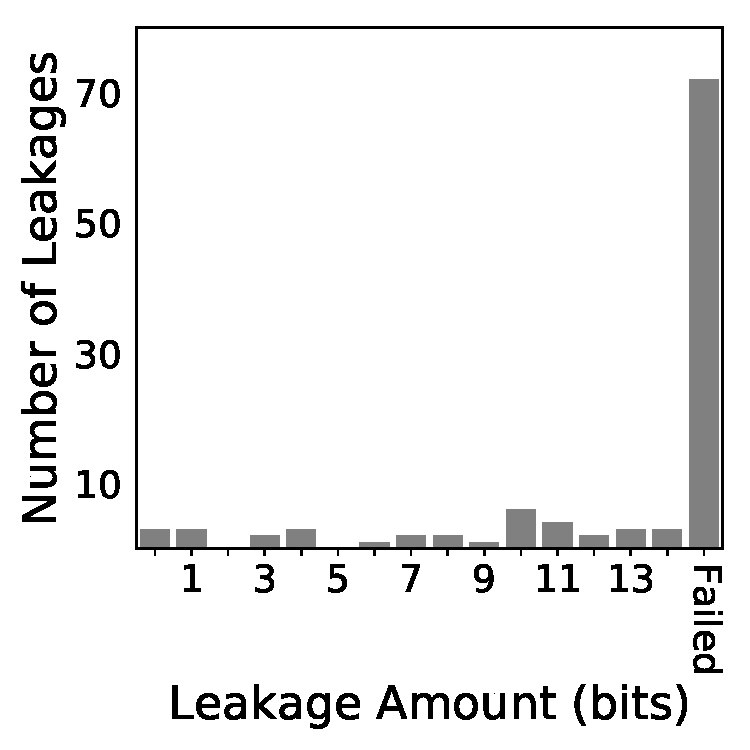
\includegraphics[width=.19\linewidth]{./figures/result/RSA-openssl-0-9-7.pdf}
    \label{fig:rsa-1}
    }
    \subfloat[RSA OpenSSL 1.0.2f]{
        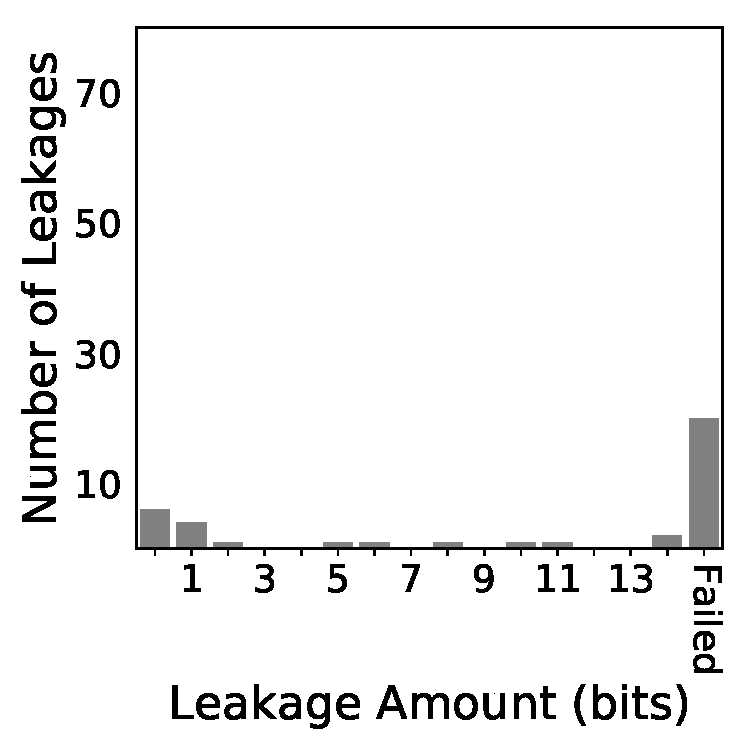
\includegraphics[width=.19\linewidth]{./figures/result/RSA-openssl-1-0-2f.pdf}
    \label{fig:rsa-2}
    }
    \subfloat[RSA OpenSSL 1.0.2k]{
        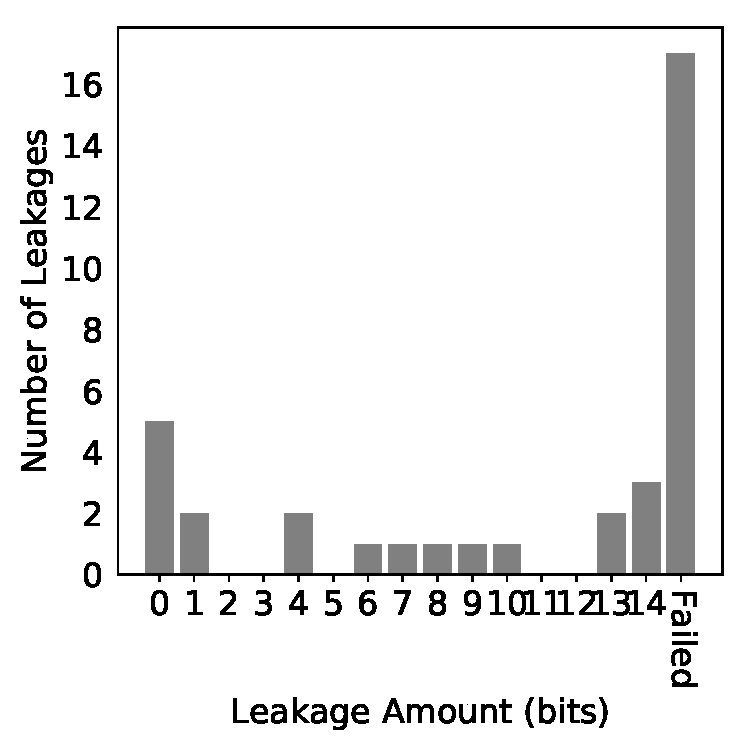
\includegraphics[width=.19\linewidth]{./figures/result/RSA-openssl-1-0-2k.pdf}
    \label{fig:rsa-3}
    }
    \subfloat[RSA OpenSSL 1.1.0f]{
        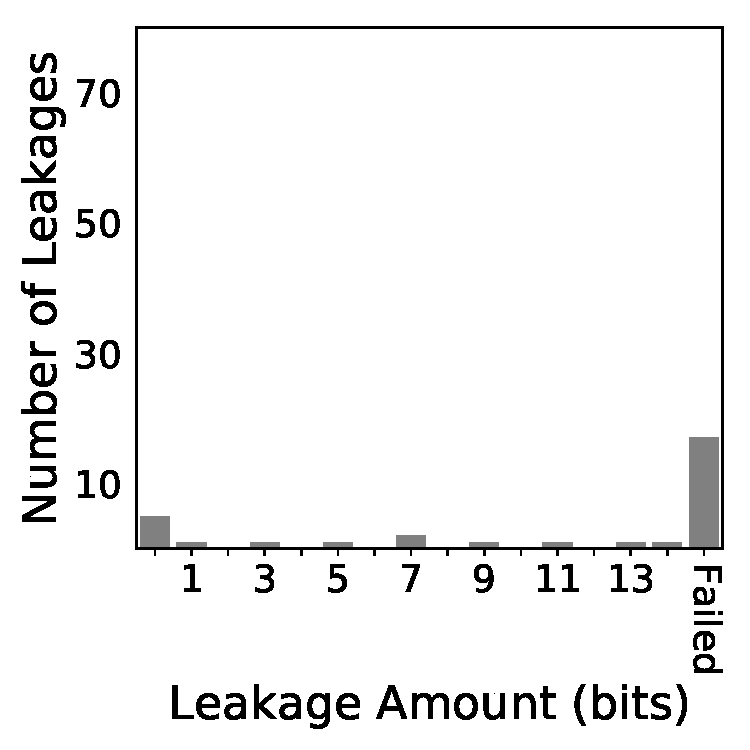
\includegraphics[width=.19\linewidth]{./figures/result/RSA-openssl-1-1-0f.pdf}
    \label{fig:rsa-4}
    }
    \subfloat[RSA OpenSSL 1.1.1]{
        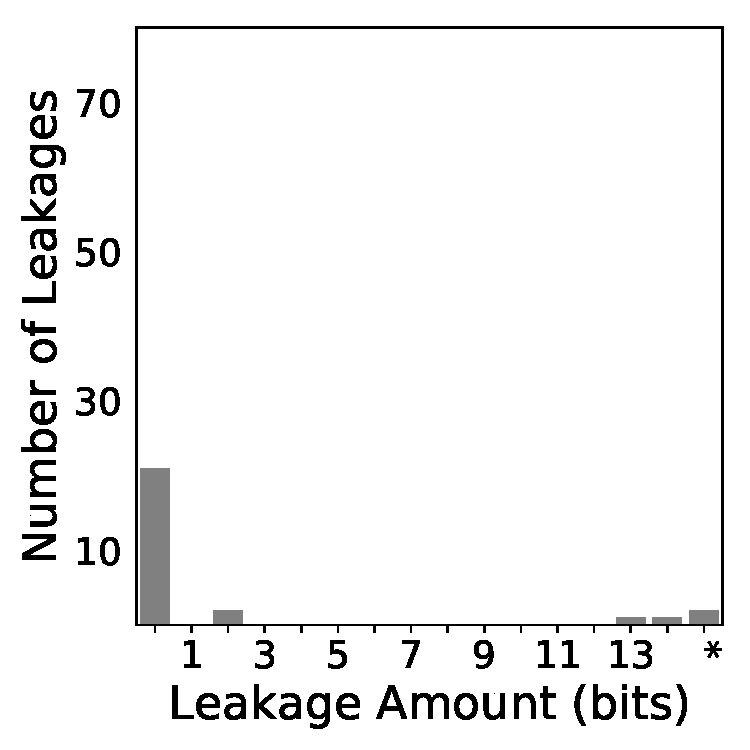
\includegraphics[width=.19\linewidth]{./figures/result/RSA-openssl-1-1-1.pdf}
    \label{fig:rsa-5}
    }
\caption{RSA implementation in different versions of OpenSSL}\label{fig:rsa}

\end{figure*}
\subsection{Analysis of Software Countermeasures}\label{sec:eval_countermeasures}
\subsubsection{Bit-slicing}
Bit-slicing is a software technology that is capable of implementing algorithms with high efficiency and constant running time. 
% Citation Needed
This approach can immune cryptographic algorithms to cache and timing-related side-channel attacks. The basic concept is to express a function in terms of single-bit logical operations (AND, XOR, OR, NOT, etc.). These operations are then carried out for multiple instances of the function in parallel, using bitwise operations on a CPU. 
% A Fast New DES Implementation in Software
% Matthew Kwan coined the term about 20 years ago after seeing Eli Biham present his paper A Fast New DES Implementation in Software. He later published Reducing the Gate Count of Bitslice DES, showing an even faster DES building on Biham’s ideas.
Matthew Kwan and Eli Biham's first present DES implements based on bit-slicing. 

\begin{figure}[h!]
    \centering
\begin{lstlisting}[xleftmargin=.02\textwidth,xrightmargin=.01\textwidth]
...
uint8_t na = ~a;
uint8_t nb = ~b;
uint8_t nc = ~c;

uint8_t t0 = (b & nc);
uint8_t t1 = (b | nc);

*l = (a & nb) | t0;
*r = (na & t1) | t0;
...
\end{lstlisting}
\caption{SBOX\_with\_BitSlicing}
\label{SBOX_bitslicing}
\end{figure}

\begin{figure}[h!]
    \centering
\begin{lstlisting}[xleftmargin=.02\textwidth,xrightmargin=.01\textwidth]
...
uint8_t SBOX[] = {1, 0, 3, 1, 2, 2, 3, 0};
x = (a << 2) + (b << 1) + c;
*l = SBOX[x] >> 1;
*r = SBOX[x] & 0b01;
...
\end{lstlisting}
\caption{SBOX\_without\_BitSlicing}
\label{SBOX_da}
\end{figure}

\subsubsection{Scatter and Gather}
The scatter-gather technology is also a common defence method to cache-based timing attacks.
\begin{figure}[h!]
    \centering
\begin{lstlisting}[xleftmargin=.02\textwidth,xrightmargin=.01\textwidth]
...
align ( buf ):
    return buf - ( buf & ( block size - 1 ) ) + block size

scatter ( buf, p, k ):
    for i := 0 to N - 1 do
        buf [k + i * spacing] := p [k][i]

gather ( r, buf, k ):
    for i := 0 to N - 1 do
        r [i] := buf [k + i * spacing]
...
\end{lstlisting}
\caption{Scatter\_and\_Gather}
\label{Scatter_and_Gather}
\end{figure}

\begin{figure}[h!]
    \centering
\begin{lstlisting}[xleftmargin=.02\textwidth,xrightmargin=.01\textwidth]
...
uint8_t SBOX[] = {1, 0, 3, 1, 2, 2, 3, 0};
align(buf);
scatter(buf, SBOX, k);

...
\end{lstlisting}
\caption{Sbox\_with\_Scatter\_and\_Gather}
\label{SBOX_sg}
\end{figure}

\subsubsection{Smaller Lookup Tables}
